\documentclass[letterpaper]{article}
\usepackage{aaai2026}
\usepackage{times}
\usepackage{helvet}
\usepackage{courier}
\usepackage[hyphens]{url}
\usepackage{graphicx}
\urlstyle{rm}
\def\UrlFont{\rm}
\usepackage{natbib}
\usepackage{caption}
\usepackage{amsmath}
\usepackage{amssymb}
\usepackage{booktabs}
\usepackage{algorithm}
\usepackage{algorithmic}
\usepackage{multirow}

\frenchspacing
\setlength{\pdfpagewidth}{8.5in}
\setlength{\pdfpageheight}{11in}

\pdfinfo{
/TemplateVersion (2026.1)
}

\title{Deep Q-Learning and Planning in Self-Play Mini-Chess:\\A Comparison of DQN, Double DQN, and MCTS}
\author{Zhenkang Dong\\
Northeastern University\\
Boston, Massachusetts 02115\\
dong.zhenk@northeastern.edu}

\begin{document}
\maketitle

% ==================================================================
\begin{abstract}
We study the application of value-based deep reinforcement learning to two-player adversarial board games by training self-play agents in 5$\times$5 Gardner Mini-Chess.
Three methods are compared under controlled conditions: Deep Q-Network (DQN), Double DQN, and Monte Carlo Tree Search (MCTS) with random rollouts.
DQN and Double DQN share identical network architectures, hyperparameters, and training budgets, isolating the effect of the target-estimation mechanism.
Agents are trained via frozen-opponent self-play and evaluated against fixed random and heuristic opponents.
We find that MCTS, requiring no training, achieves a 93\% win rate against the random opponent, far exceeding both DQN (13\%) and Double DQN (18\%).
Double DQN exhibits lower Q-value overestimation (mean $Q = 1.84$ vs.\ $1.89$) and lower cross-seed variance ($\pm 0.8\%$ vs.\ $\pm 1.4\%$) than standard DQN, confirming the theoretical prediction.
Both learned agents struggle with the sparse terminal reward structure, frequently drawing rather than winning.
We discuss the implications of these findings for applying value-based RL to adversarial games and identify reward shaping as a promising direction for improvement.
\end{abstract}


% ==================================================================
\section{Introduction}

Board games have long served as benchmark problems for artificial intelligence, from Samuel's checkers player~\cite{samuel1959} to Deep Blue~\cite{campbell2002} and AlphaGo~\cite{silver2016mastering}.
More recently, AlphaZero~\cite{silver2018general} demonstrated that a combination of Monte Carlo Tree Search and deep neural networks can achieve superhuman play across chess, shogi, and Go, all from self-play alone.
These results are impressive, but the computational resources involved---thousands of TPUs training for millions of games---place them beyond the reach of most researchers.

A natural question is whether simpler reinforcement learning methods can learn meaningful strategies in smaller-scale adversarial games.
Deep Q-Networks (DQN)~\cite{mnih2015human} have been enormously successful in single-agent settings such as Atari, but their application to two-player games introduces several complications: the environment is no longer stationary (the opponent adapts), rewards are typically sparse and terminal, and the action space may require masking for legality.

This project investigates these challenges in a controlled setting.
We use 5$\times$5 Gardner Mini-Chess~\cite{gardner1970}, a variant of chess played on a reduced board with 10 pieces per side.
Despite its smaller size, this game retains the essential strategic elements of standard chess---tactics, piece coordination, pawn promotion---and has been weakly solved with a game-theoretic value of draw~\cite{ehsan2012}.
The reduced state and action spaces make it feasible to train DQN on a single consumer GPU, while remaining complex enough that a random agent wins only a small fraction of games against any structured opponent.

We compare three methods:
\begin{enumerate}
    \item \textbf{DQN}~\cite{mnih2015human}, which serves as the baseline. We adapt DQN to the two-player setting via frozen-opponent self-play and legal-action masking.
    \item \textbf{Double DQN}~\cite{van2016deep}, which uses the identical architecture and hyperparameters as DQN but modifies the target computation to reduce overestimation bias. By holding everything else fixed, we isolate the effect of this single algorithmic change.
    \item \textbf{MCTS}~\cite{coulom2006,kocsis2006}, which is a planning-based method using UCB1 selection and random rollouts. It requires no training and serves as a non-learning reference point.
\end{enumerate}

The central question is not which method achieves the highest playing strength---MCTS with sufficient simulations will naturally dominate---but rather how DQN and Double DQN compare \emph{as learning algorithms} in terms of convergence behavior, value estimation stability, and cross-seed variance.

Our main findings are:
(1)~MCTS strongly outperforms both learned agents, highlighting the difficulty of pure value learning under sparse rewards;
(2)~Double DQN produces lower Q-value estimates and smaller overestimation bias than standard DQN, consistent with the theory of van Hasselt et al.~\cite{van2016deep};
(3)~both DQN variants converge to predominantly drawing strategies, a behavior we attribute to the combination of sparse terminal rewards and discounted value estimation.


% ==================================================================
\section{Background}

\subsection{Markov Decision Processes}

We model the agent-environment interaction as a Markov Decision Process (MDP) defined by the tuple $(\mathcal{S}, \mathcal{A}, P, R, \gamma)$, where $\mathcal{S}$ is the state space, $\mathcal{A}$ is the action space, $P(s' \mid s, a)$ is the transition function, $R(s, a)$ is the reward function, and $\gamma \in [0, 1]$ is a discount factor.
The agent seeks a policy $\pi(a \mid s)$ that maximizes the expected cumulative discounted reward $\mathbb{E}_\pi\left[\sum_{t=0}^{\infty} \gamma^t r_t\right]$.

In the two-player setting, the environment includes the opponent's behavior.
When the opponent's policy is fixed, the problem reduces to a standard (single-agent) MDP from the learning agent's perspective, though the transition dynamics are non-stationary if the opponent is periodically updated.

\subsection{Deep Q-Networks}

The action-value function $Q^\pi(s, a) = \mathbb{E}_\pi\left[\sum_{t=0}^{\infty} \gamma^t r_t \mid s_0 = s, a_0 = a\right]$ satisfies the Bellman equation:
\begin{equation}\label{eq:bellman}
    Q^*(s, a) = R(s, a) + \gamma \sum_{s'} P(s' \mid s, a) \max_{a'} Q^*(s', a').
\end{equation}
DQN~\cite{mnih2015human} approximates $Q^*$ with a neural network $Q(s, a; \theta)$ and minimizes the temporal-difference loss
\begin{equation}\label{eq:dqn-loss}
    L(\theta) = \mathbb{E}\left[\left(r + \gamma \max_{a'} Q(s', a'; \theta^{-}) - Q(s, a; \theta)\right)^2\right],
\end{equation}
where $\theta^{-}$ denotes the parameters of a periodically updated target network.
Two key ingredients stabilize learning: experience replay, which stores transitions $(s, a, r, s')$ in a buffer and samples minibatches uniformly, and the target network, which provides a slowly changing regression target.

\subsection{Double DQN}

Van Hasselt et al.~\cite{van2016deep} observed that the $\max$ operator in Equation~\ref{eq:dqn-loss} uses the same network to both \emph{select} and \emph{evaluate} the next action, inducing an upward bias in Q-value estimates.
Double DQN decouples these two operations:
\begin{equation}\label{eq:ddqn-target}
    y = r + \gamma\, Q\!\left(s',\, \arg\max_{a'} Q(s', a'; \theta);\, \theta^{-}\right).
\end{equation}
The online network $\theta$ selects the greedy action, while the target network $\theta^{-}$ evaluates it.
This simple change has been shown to reduce overestimation and improve stability in Atari benchmarks~\cite{van2016deep}.

\subsection{Monte Carlo Tree Search}

MCTS~\cite{coulom2006,kocsis2006} builds a search tree incrementally through repeated simulations.
Each simulation consists of four phases: \emph{selection} (traverse the tree using UCB1), \emph{expansion} (add a new node), \emph{rollout} (play random moves to a terminal state), and \emph{backpropagation} (update visit counts and value estimates along the path).
The UCB1 selection rule balances exploitation and exploration:
\begin{equation}\label{eq:ucb1}
    \text{UCB1}(s, a) = \frac{W(s, a)}{N(s, a)} + c \sqrt{\frac{\ln N(s)}{N(s, a)}},
\end{equation}
where $W(s, a)$ is the cumulative value, $N(s, a)$ is the visit count, and $c = \sqrt{2}$ is the exploration constant.
After all simulations, the action with the highest visit count at the root is selected.


% ==================================================================
\section{Related Work}

\textbf{Deep RL for board games.}
The most prominent application of deep RL to board games is the AlphaGo/AlphaZero family~\cite{silver2016mastering,silver2018general}, which combines MCTS with a policy-value network trained via self-play.
These systems achieve superhuman performance but require substantial compute.
Tian and Zhu~\cite{tian2015} applied convolutional networks to Go with a simpler training pipeline, showing that deep features can capture positional understanding even without search.
Lai~\cite{lai2015} trained a deep neural network to play standard chess from self-play, using a position evaluation approach rather than full MCTS integration.

\textbf{DQN in adversarial settings.}
While DQN was originally developed for single-agent Atari games~\cite{mnih2015human}, several works have explored its application to multi-agent and adversarial domains.
Tampuu et al.~\cite{tampuu2017} applied DQN to multi-agent Pong, demonstrating both cooperative and competitive behaviors.
The key adaptation for two-player games is self-play, where the agent plays against a copy of itself.
Heinrich and Silver~\cite{heinrich2016} studied deep RL in imperfect-information games, noting the difficulty of non-stationary opponent distributions.

\textbf{Mini-chess and reduced board games.}
Gardner~\cite{gardner1970} proposed the 5$\times$5 chess variant, and Ehsan and Hashemi~\cite{ehsan2012} weakly solved it, establishing the game-theoretic value as a draw.
Bhatt~\cite{bhatt2018} used a reinforcement learning approach for a mini-chess variant, and the open-source implementation we build upon provides rule enforcement for several mini-chess variants.
More broadly, reduced board games have been used as testbeds for RL algorithms when full-scale games are computationally prohibitive~\cite{lanctot2019openspiel}.


% ==================================================================
\section{Methods}

\subsection{Gardner Mini-Chess Environment}

Gardner Mini-Chess is played on a 5$\times$5 board with the following initial configuration: each side has a King, Queen, Rook, Bishop, Knight, and five Pawns, arranged in the first two rows.
Standard chess rules apply with the omission of castling and the double pawn push.
Pawns promote upon reaching the back rank.
The game terminates on checkmate (decisive result) or when a position is reached where the active player has no legal moves (stalemate, counted as draw).
We impose a 200 half-move limit to prevent infinite games; any game reaching this limit is scored as a draw.

We build on an open-source Python implementation that handles rule enforcement, move generation, and game-state management.
The environment is wrapped in a Gym-like interface that the RL agent interacts with.

\subsection{State Representation}

The board state is encoded as a $12 \times 5 \times 5$ binary tensor from the active player's perspective (canonical encoding).
Channels 0--5 represent the current player's pieces $\{$Pawn, Knight, Bishop, Rook, Queen, King$\}$; channels 6--11 represent the opponent's pieces in the same order.
When it is Black's turn, the board is rotated $180^\circ$ and the piece colors are swapped, so the network always observes the game from the same viewpoint.
This canonical representation allows a single network to play both colors.

\subsection{Action Representation}

The action space consists of $|\mathcal{A}| = 625$ discrete actions, corresponding to all from-square $\times$ to-square combinations ($25 \times 25$).
A legal-action mask $m \in \{0, 1\}^{625}$ is applied at each step: illegal actions receive $Q = -\infty$ before the $\arg\max$ during action selection.
Pawn promotion defaults to queen; underpromotion is handled by the environment when multiple promotion types share the same from-to square pair.

\subsection{DQN Architecture and Training}

Both DQN and Double DQN use the same convolutional architecture:
\begin{itemize}
    \item Conv2d($12 \to 64$, $3 \times 3$, padding=1) $\to$ BatchNorm $\to$ ReLU
    \item Conv2d($64 \to 128$, $3 \times 3$, padding=1) $\to$ BatchNorm $\to$ ReLU
    \item Conv2d($128 \to 128$, $3 \times 3$, padding=1) $\to$ BatchNorm $\to$ ReLU
    \item Flatten $\to$ FC($3200 \to 512$) $\to$ ReLU $\to$ FC($512 \to 625$)
\end{itemize}
The output layer has 625 units, one per action, representing Q-values.
Training uses Adam~\cite{kingma2014adam} with learning rate $10^{-4}$, minibatch size 256, replay buffer of capacity $10^5$ transitions, and target network updates every 1000 optimization steps.
Exploration follows a linear $\varepsilon$-greedy schedule from $\varepsilon = 1.0$ to $\varepsilon = 0.05$ over 30,000 episodes.
The discount factor is $\gamma = 0.99$.
We use Huber loss (smooth $L_1$) instead of MSE to improve robustness to large TD errors, and clamp target Q-values to $[-2, 2]$ to prevent divergence.
Gradients are clipped at $\|\nabla\| \leq 1.0$.

The only difference between the DQN and Double DQN agents is the target computation: DQN uses Equation~\ref{eq:dqn-loss}; Double DQN uses Equation~\ref{eq:ddqn-target}.

\subsection{Self-Play Training Procedure}

The training procedure operates in two phases.
During a warmup phase (episodes 1--1000), the agent plays against a purely random opponent.
After warmup, the agent transitions to self-play against a \emph{frozen} copy of its own network, which is refreshed every 500 episodes.
This frozen-opponent approach, related to fictitious self-play~\cite{heinrich2016}, provides a more stable training signal than playing against the constantly updating online network, since it keeps the effective transition dynamics approximately stationary between updates.

To mitigate first-move advantage, the agent alternates between playing White and Black on successive episodes.
The canonical state encoding ensures the network can play both sides without modification.

\subsection{MCTS Implementation}

We implement a standard MCTS with UCB1 selection (Equation~\ref{eq:ucb1}) and uniform random rollouts.
At each decision point, 200 simulations are performed.
Each simulation consists of selection, expansion of one child node, a random rollout to termination (or 200-move depth limit), and backpropagation of the result.
Values are stored from White's perspective at each node, and the selection formula is adjusted depending on the active player's color.
After all simulations, the root action with the most visits is selected.

\subsection{Evaluation Opponents}

We evaluate against two fixed opponents:
\begin{itemize}
    \item \textbf{Random}: selects uniformly among legal moves.
    \item \textbf{Heuristic}: prioritizes checking moves; if none exist, selects a random capture; otherwise plays a random legal move.
\end{itemize}
The heuristic opponent is stronger than random because it exploits immediate tactical opportunities, but it has no strategic understanding.


% ==================================================================
\section{Experiments}

\subsection{Experimental Setup}

All DQN and Double DQN experiments are run for 20,000 episodes with two random seeds (42 and 123).
Evaluation is conducted every 2,000 episodes by playing 30 games against each fixed opponent, with colors alternating.
MCTS is evaluated separately by playing 30 games against each opponent with 200 simulations per move.
All experiments are run on a single NVIDIA RTX~4060 Laptop GPU.

\subsection{Training Dynamics}

\begin{figure}[t]
    \centering
    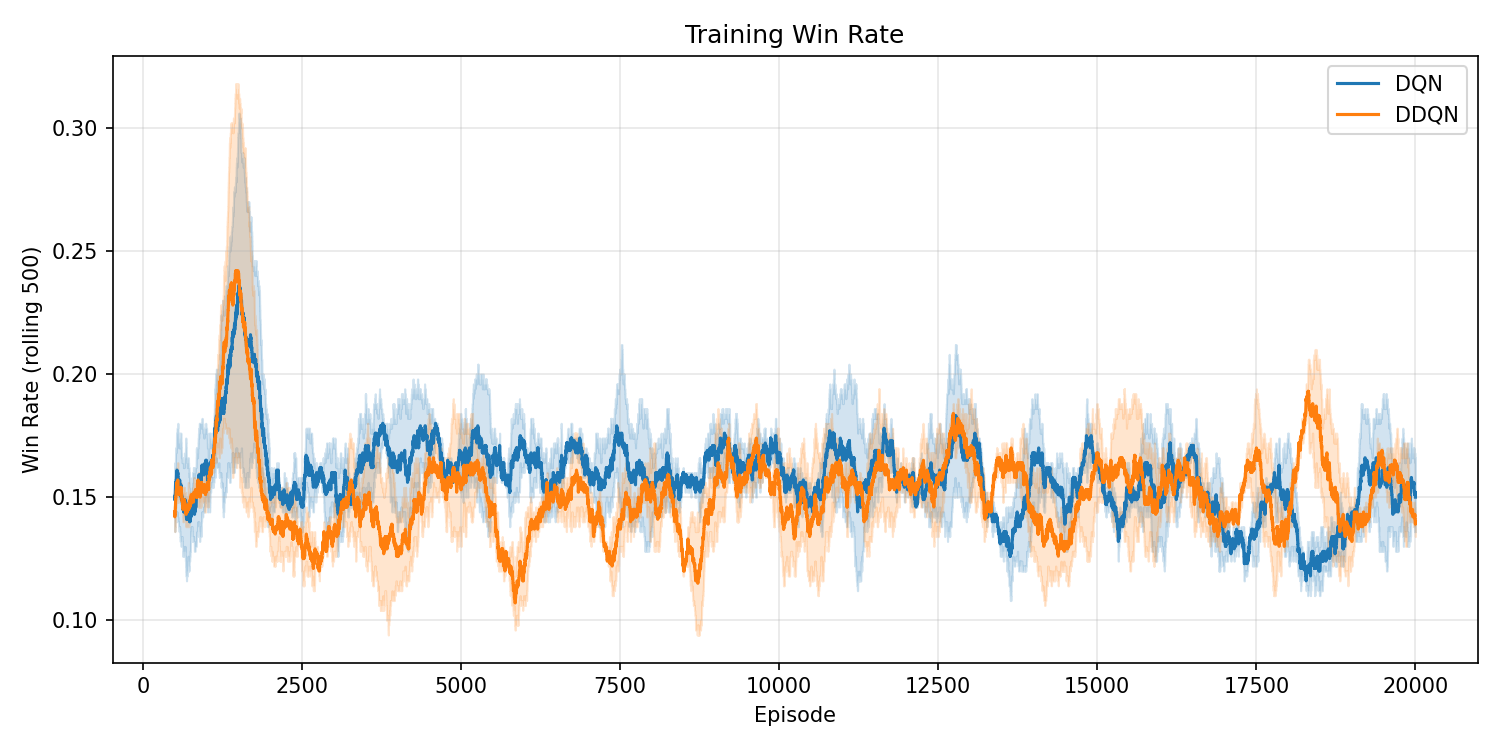
\includegraphics[width=\columnwidth]{fig_winrate.png}
    \caption{Training win rate (rolling average over 500 episodes) for DQN and Double DQN in self-play. Shaded regions indicate $\pm 1$ standard deviation across seeds.}
    \label{fig:winrate}
\end{figure}

Figure~\ref{fig:winrate} shows the training win rate over 20,000 episodes.
Both algorithms exhibit a similar trajectory: an initial rise during the warmup phase (against a random opponent), followed by a decline and stabilization after the transition to self-play at episode 1,000.
The convergent win rate of approximately 15\% reflects the difficulty of winning against a gradually improving frozen opponent---a high fraction of games end in draws.
The two methods produce comparable learning curves, with Double DQN showing marginally lower variance across seeds (visible in the shaded regions).

\begin{figure}[t]
    \centering
    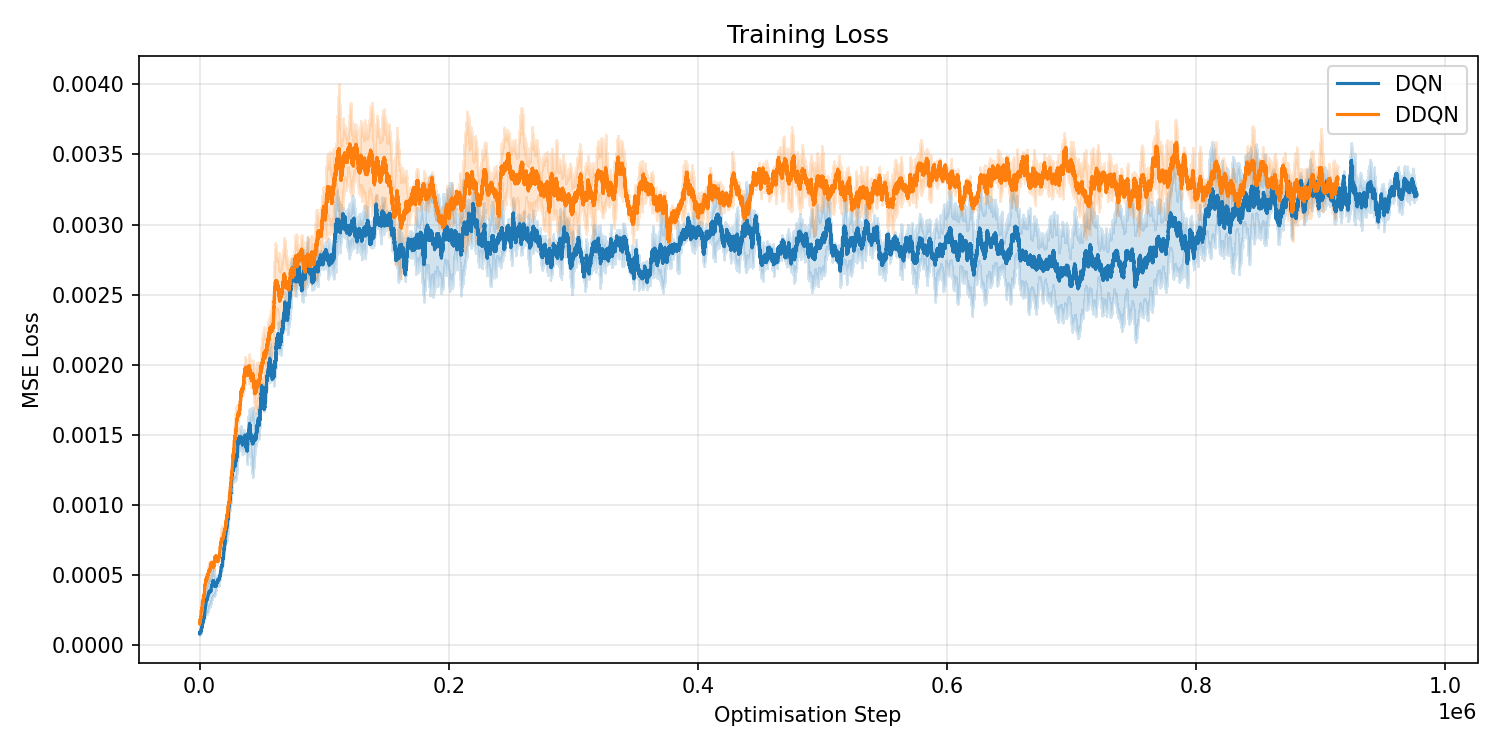
\includegraphics[width=\columnwidth]{fig_loss.png}
    \caption{Training loss (Huber) over optimization steps.}
    \label{fig:loss}
\end{figure}

The training loss (Figure~\ref{fig:loss}) converges to approximately 0.003 for both methods.
The loss increases early in training as the agent's experiences become more diverse, then stabilizes.
We note that an earlier version of our implementation using MSE loss without Q-value clamping exhibited catastrophic loss divergence (reaching $10^6$); the switch to Huber loss and target clamping resolved this.

\subsection{Q-Value Overestimation Analysis}

\begin{figure}[t]
    \centering
    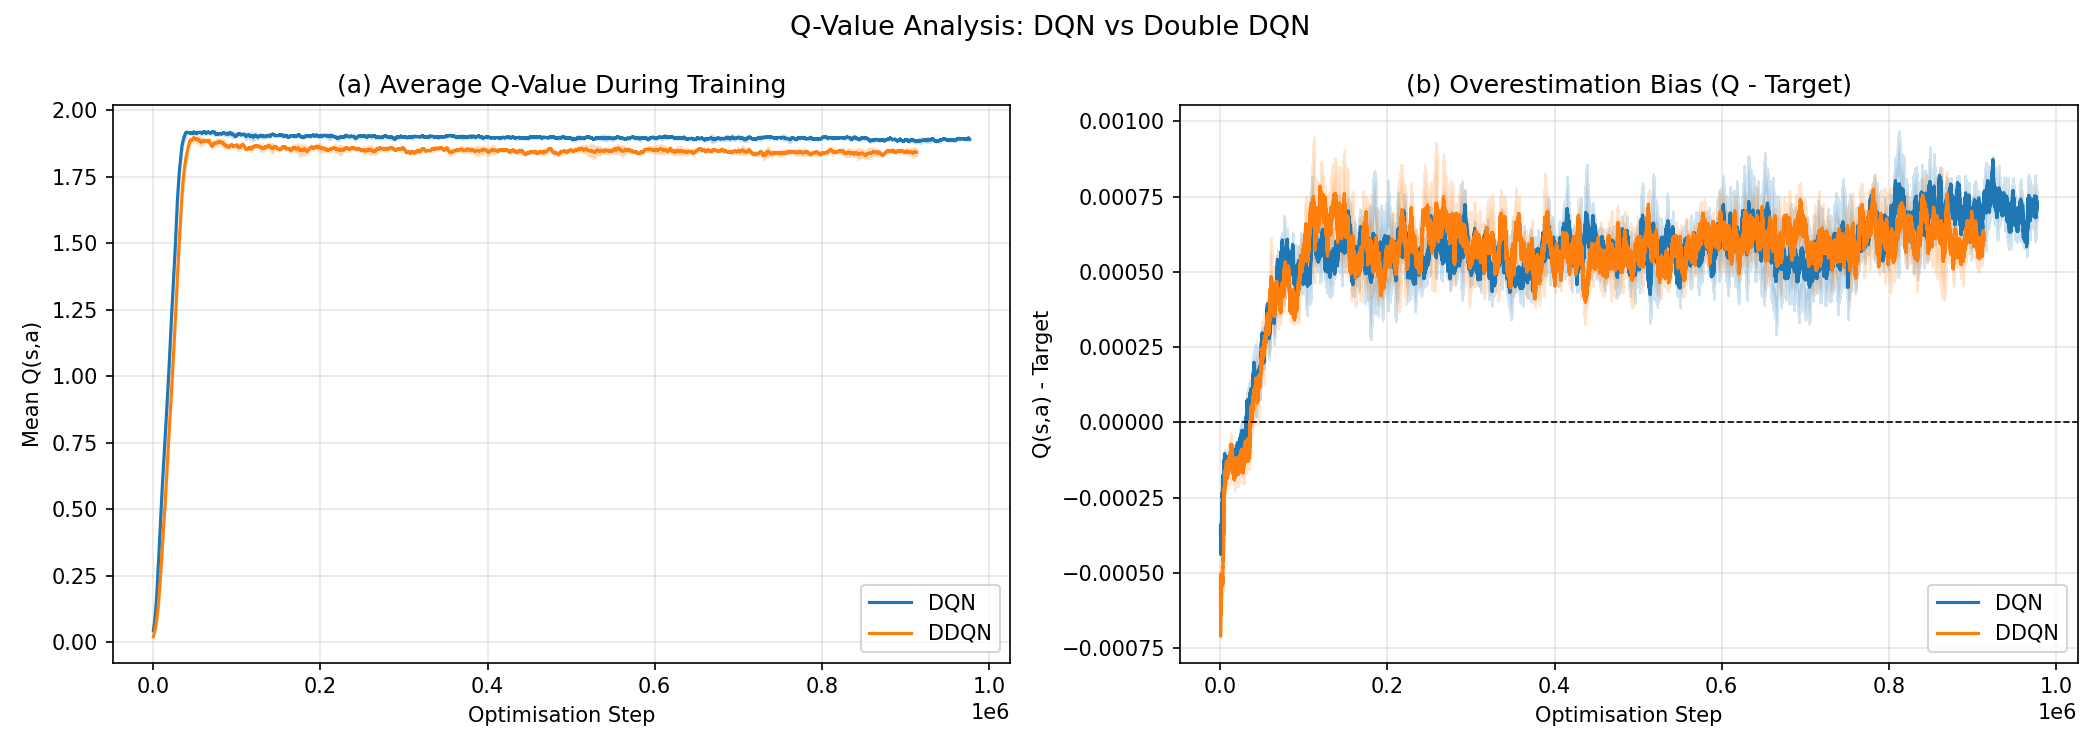
\includegraphics[width=\columnwidth]{fig_qvalues.png}
    \caption{Q-value analysis: (a) mean Q-value during training; (b) overestimation bias (Q -- target). Both are smoothed over a 2000-step window.}
    \label{fig:qvalues}
\end{figure}

The overestimation analysis (Figure~\ref{fig:qvalues}) is the central comparison of this project.
In the converged regime (last 20\% of training), DQN produces an average Q-value of 1.891 ($\pm$0.001 across seeds), while Double DQN produces 1.841 ($\pm$0.008).
The overestimation bias---defined as $\overline{Q}(s, a) - \overline{y}$, where $\overline{y}$ is the Bellman target---is $6.96 \times 10^{-4}$ for DQN and $6.16 \times 10^{-4}$ for Double DQN (Table~\ref{tab:overest}).

Although both biases are small in absolute magnitude (a consequence of the Q-value clamping to $[-2, 2]$), DQN's overestimation is consistently about 13\% larger than Double DQN's, and this difference is persistent throughout training (Figure~\ref{fig:qvalues}b).
This confirms the theoretical prediction of van Hasselt et al.~\cite{van2016deep}: the $\max$ operator in standard DQN introduces an upward bias that Double DQN mitigates by decoupling action selection from value evaluation.

\begin{table}[t]
    \centering
    \caption{Q-value statistics in the converged regime (last 20\% of training), averaged across two seeds.}
    \label{tab:overest}
    \begin{tabular}{lcc}
        \toprule
        & \textbf{DQN} & \textbf{Double DQN} \\
        \midrule
        Mean $Q(s, a)$ & 1.891 & 1.841 \\
        Mean target $y$ & 1.890 & 1.840 \\
        Overest.\ bias ($\times 10^{-4}$) & 6.96 & 6.16 \\
        Cross-seed win-rate std & $\pm 1.4\%$ & $\pm 0.8\%$ \\
        \bottomrule
    \end{tabular}
\end{table}

\subsection{Evaluation Against Fixed Opponents}

\begin{figure}[t]
    \centering
    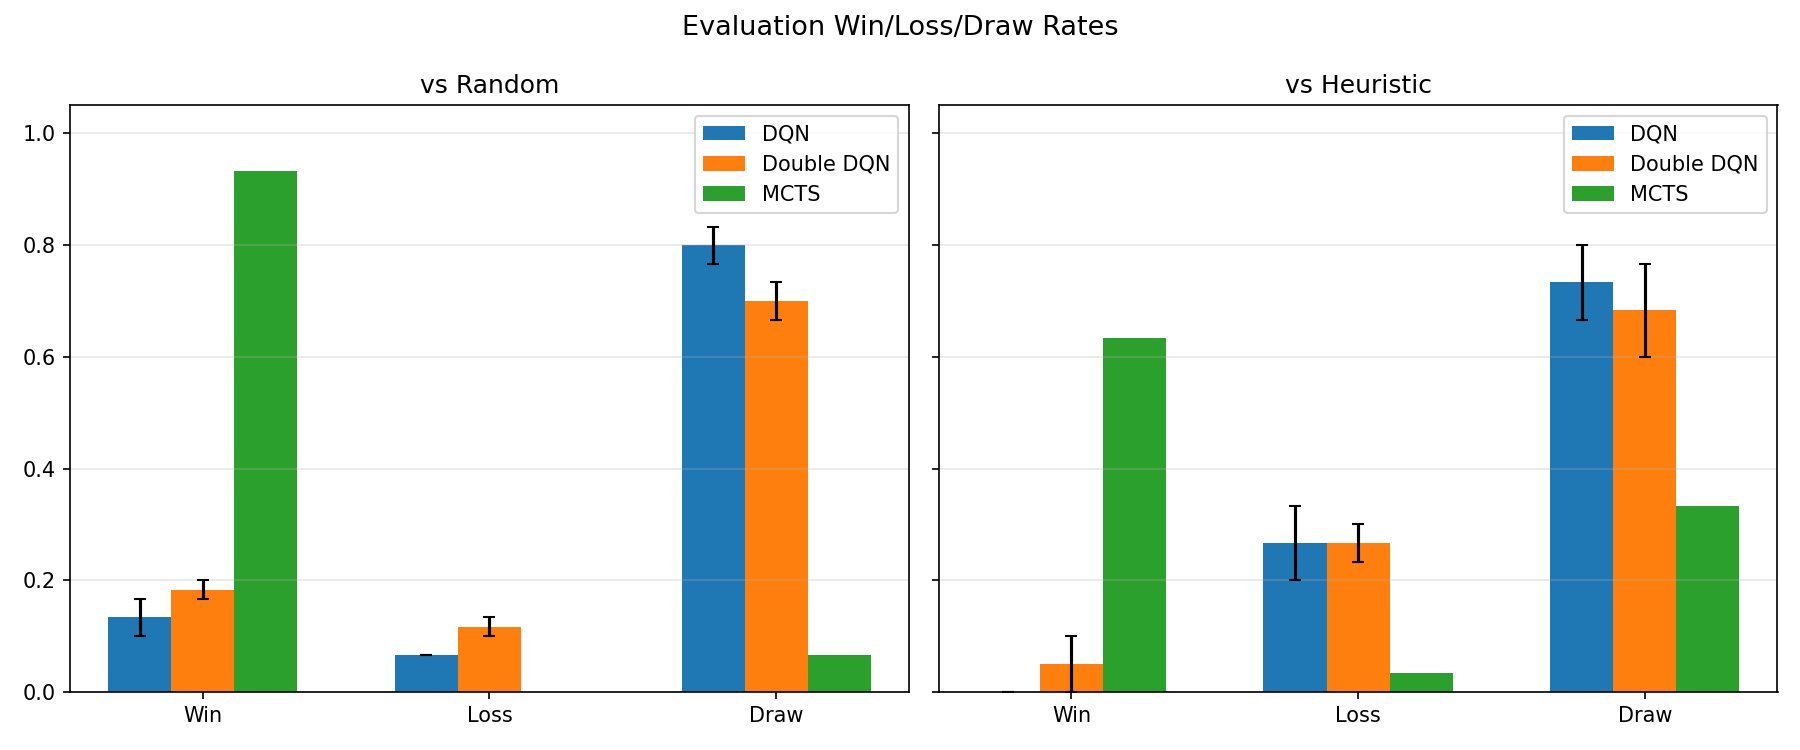
\includegraphics[width=\columnwidth]{fig_eval_bars.png}
    \caption{Win / loss / draw rates against random and heuristic opponents. DQN and Double DQN results are from the final evaluation checkpoint (episode 20,000), averaged across seeds. Error bars show $\pm 1$ std.}
    \label{fig:eval}
\end{figure}

Table~\ref{tab:eval} and Figure~\ref{fig:eval} present the evaluation results.
MCTS achieves a 93\% win rate against the random opponent and 63\% against the heuristic opponent, while never losing a single game to the random player.
Both DQN and Double DQN achieve modest win rates (13\% and 18\%, respectively) against random, with the majority of games ending in draws.
Against the heuristic opponent, neither DQN nor Double DQN wins more than 5\% of games.

\begin{table}[t]
    \centering
    \caption{Evaluation results (win / loss / draw \%) at episode 20,000, averaged across two seeds. MCTS uses 200 simulations per move.}
    \label{tab:eval}
    \small
    \begin{tabular}{@{}lccc@{}}
        \toprule
        \textbf{Opponent} & \textbf{DQN} & \textbf{DDQN} & \textbf{MCTS} \\
        \midrule
        Random (W/L/D)    & 13/7/80  & 18/12/70 & 93/0/7  \\
        Heuristic (W/L/D) & 0/27/73  & 5/27/68  & 63/3/33 \\
        \bottomrule
    \end{tabular}
\end{table}

The dominance of MCTS is expected: it performs explicit lookahead search at each decision point, which is extremely effective in a deterministic, fully observable game.
The more interesting observation is the behavior of the DQN variants.
Both agents have learned to \emph{avoid losing}---their loss rates are low---but they cannot reliably find \emph{winning} strategies.
The result is a conservative, draw-prone style of play.

\subsection{Discussion}

Several factors contribute to the limited playing strength of DQN and Double DQN:

\textbf{Sparse terminal rewards.}
The agent receives a reward signal only at the end of the game, which may be 40--50 moves away.
Under $\gamma = 0.99$, a reward 50 steps into the future is discounted by a factor of $0.99^{50} \approx 0.61$.
The network must propagate this weak signal backward through many transitions via bootstrapping, which is slow and noisy.
In contrast, MCTS evaluates positions by directly simulating games to completion, bypassing the credit-assignment problem entirely.

\textbf{Self-play non-stationarity.}
Although the frozen-opponent approach mitigates the worst forms of non-stationarity, the opponent distribution still shifts every 500 episodes.
This means the agent repeatedly faces a new effective MDP, and value estimates learned against one opponent version may be inaccurate against the next.

\textbf{Draw incentive structure.}
With terminal rewards of $+1$, $-1$, and $0$, a risk-averse policy that avoids losing (and thereby draws) is only slightly worse than a policy that sometimes wins but sometimes loses.
The value function tends to assign similar values to many states, making it difficult for the agent to differentiate winning from drawing lines of play.

\textbf{Comparison with related work.}
These challenges are well-known in the RL literature on board games.
Silver et al.~\cite{silver2018general} addressed them in AlphaZero by combining MCTS with a learned value network and using $\gamma = 1$ (no discounting).
Our results suggest that the combination of search and learning is not merely beneficial but may be \emph{necessary} for effective play in adversarial games with sparse rewards.


% ==================================================================
\section{Conclusion}

We compared DQN, Double DQN, and MCTS in 5$\times$5 Gardner Mini-Chess, a strategically rich but computationally manageable testbed for adversarial RL.
Our experiments lead to three conclusions.
First, MCTS with random rollouts substantially outperforms both DQN and Double DQN, demonstrating that explicit search provides a major advantage in deterministic games with sparse rewards.
Second, Double DQN produces lower Q-value overestimation and more stable training compared to standard DQN, confirming the theoretical analysis of van Hasselt et al.~\cite{van2016deep} in a setting quite different from Atari.
Third, both value-based methods converge to conservative, draw-heavy play, a consequence of sparse terminal rewards and the difficulty of credit assignment over long horizons.

These findings have practical implications.
For practitioners applying DQN-family algorithms to adversarial domains, our results suggest that Double DQN should be preferred over standard DQN, not because it achieves dramatically higher win rates, but because it provides more stable and predictable training dynamics.
More fundamentally, the gap between MCTS and the learned agents underscores the importance of search in game-playing AI, and motivates future work on hybrid approaches.

Several limitations should be acknowledged.
We used only two random seeds, limiting statistical power.
The training budget of 20,000 episodes may be insufficient for full convergence.
The Q-value clamping, while stabilizing, reduces the sensitivity of the overestimation analysis.
Future work should explore reward shaping (intermediate rewards for captures, checks, or material advantage), undiscounted returns ($\gamma = 1$), prioritized experience replay, and the integration of learned value functions with MCTS in the style of AlphaZero.


\bibliographystyle{aaai2026}
\bibliography{references}

\end{document}
